% \RequirePackage[l2tabu, orthodox]{nag}
% \documentclass{article}

% % FONTS
\usepackage[T1]{fontenc}

% Replace default Latin Modern typewriter with its proportional counterpart
% http://www.tug.dk/FontCatalogue/lmoderntypewriterprop/
\renewcommand*\ttdefault{lmvtt}

%\usepackage[bitstream-charter]{mathdesign} % not needed for mtpro
\usepackage{amsmath}
\usepackage[subscriptcorrection,
            amssymbols,
            mtpbb,
            mtpcal,
            nofontinfo  % suppresses all warnings
           ]{mtpro2} %TODO: put htis back in and take out mathdesign
\usepackage{scalefnt,letltxmacro}
\LetLtxMacro{\oldtextsc}{\textsc}
\renewcommand{\textsc}[1]{\oldtextsc{\scalefont{1.10}#1}}
\usepackage[scaled=0.92]{PTSans}


% % COLOR
\usepackage[usenames,dvipsnames]{xcolor}
\definecolor{Green}{HTML}{156946}

% % SPACING and TEXT
\usepackage[final,expansion=alltext]{microtype}
\usepackage[english]{babel}
\usepackage{afterpage}
\usepackage{framed}


% define a paragraph header function
\DeclareRobustCommand{\parhead}[1]{\textbf{#1}~}

% % EDITING
% paragraph helper
\DeclareRobustCommand{\PP}{\textcolor{Plum}{\P} }

% % COUNTERS
\usepackage{enumitem}
\renewcommand{\labelenumi}{\color{black!67}{\arabic{enumi}.}}
\renewcommand{\labelenumii}{{\color{black!67}(\alph{enumii})}}
\renewcommand{\labelitemi}{{\color{black!67}\tiny$\blacksquare$}}
\renewcommand{\labelitemii}{{\color{black!67}\textbullet}}
\renewcommand{\labelitemiii}{{\color{black!67}\scriptsize$\blacktriangleright$}}

% FIGURES
\usepackage{graphicx}

% TABLES
\usepackage{booktabs}

% ALGORITHMS
\usepackage[algoruled]{algorithm2e}
\usepackage{listings}
\usepackage{fancyvrb}
\fvset{fontsize=\normalsize}

% % HYPERREF
\usepackage[colorlinks,linktoc=all]{hyperref} %TODO: rm draft
\usepackage[all]{hypcap}
\hypersetup{citecolor=Green}
\hypersetup{linkcolor=Green}
\hypersetup{urlcolor=Green}

% % CLEVEREF must come after HYPERREF
\usepackage[nameinlink]{cleveref}

% BIBLIOGRPHY: get rid of reference labels
\makeatletter
	\renewcommand\@biblabel[1]{}
\makeatother

% ACRONYMS
\usepackage[acronym,smallcaps,nowarn]{glossaries}
% \makeglossaries

% % COLOR DEFINITIONS
\newcommand{\green}[1]{\textcolor{Green}{#1}}


% LISTINGS DEFINTIONS
\lstdefinestyle{mystyle}{
    commentstyle=\color{Green},
    keywordstyle=\color{Green},
    numberstyle=\tiny\color{black!60},
    stringstyle=\color{Green},
    basicstyle=\ttfamily,
    breakatwhitespace=false,
    breaklines=true,
    captionpos=b,
    keepspaces=true,
    numbers=left,
    numbersep=5pt,
    showspaces=false,
    showstringspaces=false,
    showtabs=false,
    tabsize=2
}
\lstset{style=mystyle}

% ALGORITHMS
\usepackage[algoruled]{algorithm2e}

% FRAMES
\usepackage[linewidth=1pt]{mdframed}
\DeclareRobustCommand{\mb}[1]{\ensuremath{\boldsymbol{\mathbf{#1}}}}

\DeclareMathOperator*{\argmax}{arg\,max}
\DeclareMathOperator*{\argmin}{arg\,min}

\DeclareRobustCommand{\KL}[2]{\ensuremath{\textrm{KL}\left(#1\;\|\;#2\right)}}

\newcommand{\mbx}{\mathbold{x}}
\newcommand{\mbX}{\mbf{X}}

\newcommand{\mbz}{\mathbold{z}}

\newcommand{\mbI}{\mbf{I}}

\newcommand{\mbZ}{\mbf{Z}}
\newcommand{\mbL}{\mbf{L}}

\newcommand{\mbtheta}{\mathbold{\theta}}
\newcommand{\mbTheta}{\mathbold{\Theta}}
\newcommand{\mbomega}{\mathbold{\omega}}
\newcommand{\mbOmega}{\mathbold{\Omega}}
\newcommand{\mbsigma}{\mathbold{\sigma}}
\newcommand{\mbSigma}{\mathbold{\Sigma}}

\newcommand{\mblambda}{\mathbold{\lambda}}
\newcommand{\mbgamma}{\mathbold{\gamma}}
\newcommand{\mbzeta}{\mathbold{\zeta}}
\newcommand{\mbeta}{\mathbold{\eta}}
\newcommand{\mbbeta}{\mathbold{\beta}}
\newcommand{\mbphi}{\mathbold{\phi}}
\newcommand{\mbmu}{\mathbold{\mu}}
\newcommand{\mbrho}{\mathbold{\rho}}

\newcommand\dif{\mathop{}\!\mathrm{d}}
\newcommand{\diag}{\textrm{diag}}
\newcommand{\supp}{\textrm{supp}}

\newcommand{\E}{\mathbb{E}}
\newcommand{\Var}{\mathbb{V}\textrm{ar}}

\newcommand{\bbN}{\mathbb{N}}
\newcommand{\bbZ}{\mathbb{Z}}
\newcommand{\bbR}{\mathbb{R}}
\newcommand{\bbS}{\mathbb{S}}

\newcommand{\cL}{\mathcal{L}}

\newcommand{\cN}{\mathcal{N}}
\newcommand{\Gam}{\textrm{Gam}}
\newcommand{\InvGam}{\textrm{InvGam}}

\newcommand{\g}{~\vert~}
\newacronym{KL}{kl}{Kullback-Leibler}
\newacronym{ELBO}{elbo}{\emph{evidence lower bound}}
\newacronym{POPELBO}{pop-elbo}{\emph{population evidence lower bound}}

\newacronym{SVI}{svi}{stochastic variational inference}
\newacronym{BUMPVI}{bump-vi}{bumping variational inference}

\newacronym{GMM}{gmm}{Gaussian mixture model}
\newacronym{LDA}{lda}{latent Dirichlet allocation}

\newacronym{SUTVA}{sutva}{stable unit treatment value assumption}

% fanciness for quote
\usepackage{epigraph}
\patchcmd{\epigraph}{\@epitext{#1}}{\itshape\@epitext{#1}}{}{}

\begin{document}

\title{Who, What, When, Where, and Why? \\ A Computational Approach to Understanding Historical Events Using State Department Cables}

\author{Allison J.B. Chaney, Hanna Wallach, David M. Blei}

\maketitle

\vspace{0.3in}

\begin{center}
\parbox{3.5in}{
\raggedright{
 	\emph{We can do nothing but scrutinize historical events themselves if we want to discover what they are.}}\\
\smallskip
\raggedleft{-- Dean W.R. Matthews, \emph{What is an Historical Event?}}
}
\end{center}

\vspace{0.5in}

\begin{abstract}
	We develop computational methods for analyzing historical documents to identify events of potential historical significance. Significant events are characterized by interactions between entities (e.g., countries, organizations, individuals) that deviate from typical interaction patterns. When studying historical events, historians and political scientists commonly read large quantities of text to construct an accurate picture of who, what, when, and where---a necessary precursor to answering the more nuanced question, ``Why?'' Our methods help historians identify possible events from the texts of historical communication. Specifically, we build on topic modeling to distinguish between topics that describe ``business-as-usual'' and topics that deviate from these patterns, where deviations are also indicated by particular entities interacting during particular periods of time. To demonstrate our methods, we analyze a corpus of 2 million State Department cables from 1973 to 1977.  For example, we show that we are able to detect and characterize the Fall of Saigon.
\end{abstract}


\section{Introduction}

Communications between the U.S. State Department and its embassies have historically been called \emph{diplomatic cables}, derived from the time when physical cables were used for such communications.
We obtained around two million of these cables sent between 1973 and 1977 via the History Lab at Columbia,\footnote{http://history-lab.org} which received them from the Central Foreign Policy Files at the National Archives.  In addition to the text of the cables themselves, each document is supplemented with information about who sent the cable (e.g., the State Department, the U.S. Embassy in Saigon, or an individual by name), who received the message (often multiple entities), and the date the message was sent.
Figure~\ref{fig:cables_example} shows three cables which were sent in April 1975 concerning orphans from the Vietnam War.


\begin{figure}[ht]
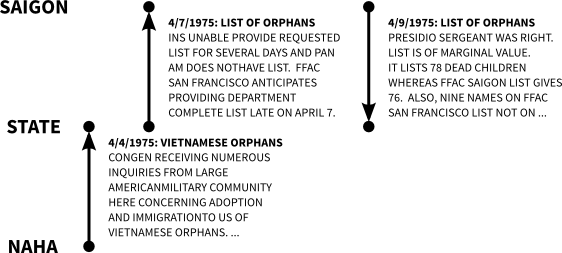
\includegraphics[width=\textwidth]{fig/cables_orphan_example.png}
\caption{Example excerpts of cables.}
\label{fig:cables_example}
\end{figure}

Historians and political scientists are interested in the process of sending cables---of particular interest is identifying historical events in a collection of these cables.  These experts want to know \emph{when} events happen, as well as \emph{what} happens during the event, which includes the parties sending and receiving messages (\emph{who}). 

For this work, we characterize an event in two ways: \emph{when} it occurs and \emph{what} occurs.  We assume that only one event can begin on any given day, which allows us to describe each day in terms of the probability of an event starting that day.  We can also assume that an event will influence cables for a set time period after it starts---this way, we only need to discover the starting day for each event.  
To understand \emph{what} occurs, we can summarize the cable message content with a topic model such as LDA~\citep{Blei:2003} and model event content in that same space.


\section{A Generative Model of Events}
Our model is a generative process---we make assumptions about how the data came to be and describe these assumptions in terms of probability distributions.  Given our model and observed data, the task is then to reverse the generative process to find the hidden quantities that (retrospectively) generated the data.

Consider an entity like the Bangkok American embassy.  We can imagine that there is a stream of cables being sent by this embassy---some might be sent to the US State Department, others to another American embassy like Hong Kong, and perhaps a few are sent to individuals by name.  Each of these cables has an associated send date, and we can represent the content of the cable with a topic model; we call these cable descriptions $\theta$, which is a matrix of $D$ cables (or documents) by $K$ topics.\footnote{This allows us to represent the cable in terms of about 100 topics rather than in terms of hundreds of thousands of vocabulary words. We can discover these topics with LDA and treat them as fixed observations going forward.}

An entity will usually talk about certain topics and with certain frequency. The Bangkok embassy, for instance, sent and average of 22 cables per day in the 1970s, and was concerned with topics regarding southeast Asia more generally.  We can describe the general interests of entities in the same topic space we use to describe individual cables and we will call these per-entity interests $\phi$ and can assign them a formal distribution.
\begin{itemize}
\item Draw the entity's base topics: $\phi_{0k} \sim \mbox{Gamma}(\alpha, \beta)$
\end{itemize}
Eventually we will want to model the interactions between entities, but for now we can consider a single entity at a time.

Now imagine that at a particular time, an event occurs, such as the capture of Saigon during the Vietnam war.  We do not directly observe that events occurs, but each event can again be described in the same topic space used to describe individual cables.  Whether or not an event occurs at a particular time step is represented by $\epsilon_t$ and the content of the event (or its topical representation) is called $\pi_t$.

\begin{itemize}
\item For each day $i$ with date $a_i$:
\begin{itemize}
\item Generate event occurrence/strength $\epsilon \sim \mbox{Poisson}
(\eta_\epsilon)$, where $\eta_\epsilon$ is a fixed, non-negative
hyperparameter for the mean event strength.
\item Generate the day/event's description in terms of each topic $k$: $\pi_{ik} \sim \mbox{Gamma}(\alpha_0, \beta_0)$, where $\alpha_0$ and $\beta_0$ are fixed hyperparameters.
\end{itemize}
\end{itemize}

When an event occurs, both the frequency of cables being sent and the cable content changes. The Bangkok embassy sent 31 cables the day following the capture of Saigon (a 36\% increase over the average), and the majority of these cables are about Vietnam war refugees.  Thus we imagine that an entity's stream of cables is controlled by what it usually talks about (and how often) as well as the higher level stream of unobserved events.  The influence of an event does not last indefinitely, however, so we model the decay of its magnitude with some function $f$.
While many decay functions can be used, we define the event decay function to be a simple linear decrease: \[f(a, c) =
\begin{cases}
	1 - \frac{c-a}{d}, & \mbox{if } a \le c < a+d \\
	0, & \mbox{otherwise,}
\end{cases} \]
where $d$ is the time distance (in days) after event $a$ at which point the event is no longer relevant.

When we analyze the cables with this model setup, we disentangle cables that represent ``business as usual'' from those that reflect the higher-order event stream.  Consequently, we infer what that stream is,
i.e., when something happened and what happened.

Recall that the key hidden values are event descriptions $\pi$ (``what''), event occurrences $\epsilon$ (``when''), and entity interests $\phi$.  (Since entities are tied to individuals and places, we can use them to describe ``who'' is involved and ``where'' and event occurs after fitting our model.)  These are all tied together when we model the observed data itself, as we assume that each cable is generated from a combination of these parameters.
\begin{itemize}
\item For each cable $j$ on date $c_j$:
\begin{itemize}
	\item Set cable topic parameter: $\phi_{jk} = \phi_{0k} + \sum_i f(a_i, c_j) \pi_{ik} \epsilon_i$.
	\item Draw cable topic: $\theta_{jk} \sim \mbox{Gamma}(\beta_c \phi_{jk}, \beta_c)$.
\end{itemize}
\end{itemize}



\subsection{Inference}
Posterior inference is the central computational problem.  We want to learn the hidden values describe above (event descriptions $\pi$, event occurrences $\epsilon$, and entity descriptions $\phi$) from our observed data.  We construct a black box variational inference algorithm following~\citet{Ranganath:2014} to determine the values of these latent parameters.

\section{Validation}
TODO

\section{Discussion}
Once we have determined the values of the hidden parameters in our model, we will have a discrete list of events in terms of when they occur and their topical content.  We plan to compare these discovered events to a list of predetermined historical events to evaluate the effectiveness of our model.

Traditional topic models can describe documents, but they cannot identify when events occur---only a model like ours that explicitly models event occurrences and event content can attribute document observations to discrete events.  Further, by modeling entities, we can distinguish between ``business-as-usual'' document content and content that is attached to particular events---we are also unable to capture this phenomenon with traditional topic models.

%needs vlaidation: how to check our model is doing what we want; compare to real, known, events



\bibliographystyle{apa}
\bibliography{/Users/ajbc/Dropbox/papers/library.bib}

\end{document}
